\documentclass[tikz, border=5mm]{standalone}
\usepackage{textcomp}
\usetikzlibrary{arrows.meta,decorations.markings,fit,calc, positioning}

\definecolor{componentColor}{RGB}{210,210,210}
\definecolor{systemColor}{RGB}{230,230,230}

\tikzset{component/.append style={fill=componentColor, align=center, draw, minimum width=2cm, minimum height=1.5cm, rounded corners=.3cm}}
\tikzset{system/.style={ component, fill=systemColor, rounded corners=0cm}}


\begin{document}
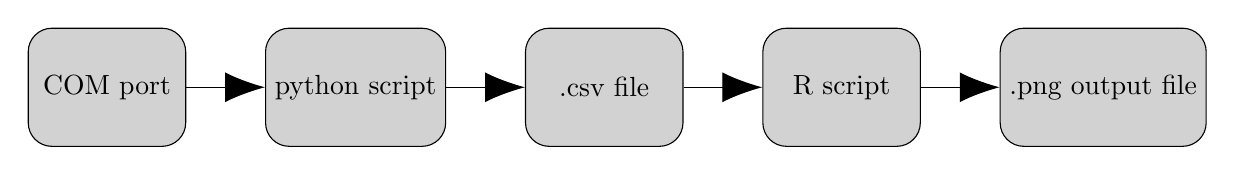
\begin{tikzpicture}[node distance=0.3cm and 1cm]

    % Nodes
    \node (a0) [component] {COM port};
    \node (a1) [component, right=of a0] {python script};
    \node (a2) [component,right=of a1] {.csv file};
    \node (a3) [component,right=of a2] {R script};
    \node (a4) [component,right=of a3] {.png output file};

    % Connectors
    \begin{scope}[->]

        \draw [-{Latex[scale=3.0]}] (a0) -- node[anchor=west, minimum height=.25cm, draw=none]{} (a1);
        \draw [-{Latex[scale=3.0]}] (a1) -- node[anchor=west, minimum height=.25cm, draw=none]{} (a2);
        \draw [-{Latex[scale=3.0]}] (a2) -- node[anchor=west, minimum height=.25cm, draw=none]{} (a3);
        \draw [-{Latex[scale=3.0]}] (a3) -- node[anchor=west, minimum height=.25cm, draw=none]{} (a4);

    \end{scope}

\end{tikzpicture}
\end{document}
